\documentclass[11pt]{article}

\usepackage[utf8]{inputenc}
\usepackage[T1]{fontenc}
\usepackage{lmodern}
\usepackage[margin=1in]{geometry}
\usepackage{amsmath,amssymb}
\usepackage{graphicx}
\usepackage{booktabs}
\usepackage{microtype}
\usepackage{xcolor}
\usepackage{caption}
\usepackage[hidelinks]{hyperref}
\usepackage{enumitem}
\graphicspath{{figures/}}
\captionsetup{font=small,labelfont=bf}

\title{\textbf{Action-Coupled, Cost-Bounded Memory for Multi-Tenant Agents}\\[4pt]
\large FERNme --- a user-owned, near-zero-LLM Hebbian preference-graph memory}

\author{Mirkomil Sharipov\\ Acquilab Inc.\\ \texttt{mirkosharipov@acquilab.io}}
\date{Preprint draft (system v0.1.0)}

\begin{document}
\maketitle

\begin{abstract}
\noindent LLM-agent memory systems have converged on graph- and activation-based
designs that improve long-horizon recall, but they share three properties that are
limiting for agents that \emph{act for many people}: memory is \textbf{written by
per-interaction LLM extraction} (costly and error-prone), it is \textbf{evaluated on
question answering} rather than on actions taken, and it assumes a
\textbf{single-user, single-deployment} setting. We present \textbf{FERNme}
(Fuzzy-Edged Recall Network), a memory layer for multi-tenant agents in which each
user is a sparse, fuzzily-weighted node (single-digit $0$--$9$ edges) in a per-surface
preference graph. Edges are updated by a \textbf{Hebbian co-occurrence rule with no
per-interaction LLM call}, retrieved by spreading activation, and compiled to a
token-minimal ``card'' via \textbf{differential encoding} (storing only deviations
from a population prior). Memory is coupled to the agent's action layer, gated by
uncertainty, user-owned, consent-first, and glass-box editable; a user signs in across
surfaces (web today; desktop and mobile on the roadmap) to assemble a cross-surface
\textbf{supernode} they control. Across reproducible simulations we show that (i)
per-turn token cost stays \textbf{flat} as a profile grows ($\approx 25$ tokens; a
full-history baseline is $77\times$ larger by $120$ interactions) at \textbf{zero}
write-time LLM calls; (ii) FERNme matches a frequency baseline on stationary
preferences while \textbf{substantially outperforming it under preference drift}
($0.72$ vs.\ $0.13$ precision@5) and on \textbf{context-conditioned} retrieval ($0.62$
vs.\ $0.51$); and (iii) in a simulated storefront, FERNme-personalized recommendations
yield a \textbf{+16\% relative conversion lift}. We further validate the engine on a
\textbf{natural single-user dataset} --- 86 free-form diary entries about one fictional
person --- where FERNme ingests every entry with \textbf{0 write-time LLM calls}, holds
a \textbf{flat ${\sim}40$-token card}, \textbf{retains 16/16} of the person's stated
permanent facts, exhibits correct \textbf{preference drift}, and uses \textbf{${\sim}10\times$
/ ${\sim}240\times$ fewer tokens} than extraction-based and full-history memory
respectively. On a LoCoMo-style QA set, FERNme's context-seeded retrieval answers
\textbf{${\sim}4\times$} as many fact questions as frequency/recency baselines at equal
budget and is the only LLM-free method that resolves preference drift. We argue that for
agents that act for many users, memory should be \textbf{cheap to write} and
\textbf{evaluated by outcomes}, and that a user-owned, per-surface design is both a
cleaner trust contract and a defensible deployment model.
\end{abstract}

\section{Introduction}
Conversational assistants are giving way to agents that \emph{act} on a user's behalf
--- buying, booking, applying, routing, and increasingly doing so across a website, a
desktop app, and a phone. Memory is central to making such agents useful across visits
and surfaces, but the dominant designs were built for a different problem. They (1)
write memory by invoking an LLM to extract and reconcile facts on every interaction,
which is expensive at scale and introduces a write-time hallucination surface; (2) are
benchmarked on question-answering, which measures recall, not whether the agent did the
right thing; and (3) assume one user and one deployment, with no notion of per-tenant
isolation, ownership, or consent.

For a memory that sits behind an agent serving \emph{many} people and \emph{acting} on
their behalf, the priorities invert. Writes must be cheap because they happen
constantly. Success is an action outcome (a completed purchase, a re-order, a filled
booking), not a QA score. And because the memory holds personal data, isolation,
consent, and user control are first-class requirements.

\paragraph{Contributions.}
\begin{enumerate}[leftmargin=1.4em,itemsep=2pt]
\item \textbf{A memory-write mechanism with no per-interaction LLM call} --- a
saturating Hebbian co-occurrence update over a fuzzy ($0$--$9$) preference graph, with
ACT-R-style decay and explicit negative edges --- targeting the cost and reliability
weaknesses of extraction-based memory.
\item \textbf{Differential, population-prior encoding} as an agent-memory token
mechanism: a new user inherits a population baseline and we store only deviations,
giving a small, bounded card and a modest cold-start benefit, with $k$-anonymity and
differential privacy on the shared prior.
\item \textbf{An action-coupled framing and an outcome-oriented evaluation} ---
including a simulated storefront that scores conversion lift --- alongside an analysis
of where a cheap counter-style memory wins and loses (static vs.\ drift vs.\ context).
\item \textbf{A multi-tenant, user-owned design} --- per-surface isolation, consent
gating, glass-box editing and a memory-graph view, and an opt-in cross-surface
\emph{supernode} assembled by user sign-in with default-deny scoped sharing.
\item \textbf{An evaluation on natural, free-form single-user data} (Section~\ref{sec:elena})
that validates the storage, reinforcement, decay, confidence, drift, and flat-cost
mechanics on text not written for clean extraction, including a LoCoMo-style QA
head-to-head.
\end{enumerate}

We are explicit about positioning: the graph + spreading-activation \emph{mechanism} is
not novel (Section~\ref{sec:related}), and on stationary recall FERNme merely ties a
frequency baseline (Section~\ref{sec:results}). The contribution is the
\emph{combination} --- cheap writes, outcome evaluation, a private collective prior, and
a user-owned per-surface contract.

\section{Related work}\label{sec:related}
The engine's mechanism family --- Hebbian co-occurrence, ACT-R-style activation decay,
and spreading activation over a graph --- is \emph{shared, public cognitive-science
machinery}, and several recent systems use it. We do not claim the mechanism; we claim
the surrounding system.

\paragraph{Spreading-activation / Hebbian memory (closest mechanism).} HippoRAG and
HippoRAG~2~\cite{hipporag,hipporag2} formalize associative retrieval over a knowledge
graph via Personalized PageRank, but as a \emph{document-retrieval} framework (LLM-based
OpenIE indexing + embeddings). \emph{Ori-Mnemos}~\cite{ori} packages ACT-R decay,
spreading activation, and Hebbian co-occurrence as a sovereign single-agent note vault.
\emph{HeLa-Mem}~\cite{helamem} builds a Hebbian graph over a single user's conversation
with LLM-based ``Hebbian Distillation.'' FERNme uses the same retrieval family but
differs in purpose (personalization \emph{about end-users}, evaluated on actions), write
rule (no LLM on the hot path), and deployment (multi-tenant, user-owned, with a private
collective prior). Its memory is about \emph{whom the agent serves}, not the agent's own
knowledge.

\paragraph{Extraction-based / production memory.} Mem0~\cite{mem0} writes memory by LLM
extraction and reconciliation per interaction and retrieves by vector similarity,
benchmarked on conversational QA. This is \emph{smarter per write} --- it captures
nuanced, causal preferences a co-occurrence counter misses --- but it is costly and adds
a write-time error surface. FERNme trades that richness for a near-zero write cost and
makes the trade-off explicit (recoverable via optional gated/offline modes).

\paragraph{Tiered, temporal, and classical.} MemGPT/Letta and MemoryOS manage context in
LLM-paged tiers; Zep/Graphiti track fact validity over time with a temporal knowledge
graph. FERNme's tiers (Card / Cabinet / baked-in defaults) serve token bounding for a
live action loop, and it handles non-stationarity with decay rather than an explicit
temporal graph. FERNme is an elaboration of well-established ideas: spreading
activation~\cite{collins1975spreading,anderson2004actr}, Hebbian learning~\cite{hebb1949},
fuzzy sets~\cite{zadeh1965}, and vector-space / IDF weighting. We claim none of these as
new.

\section{Method}
\paragraph{Substrate.} Each user is a node connected to attribute nodes
(\texttt{pref:organic}, \texttt{!pref:upsells}, \dots) by edges carrying a continuous
strength in $[0,9]$ (a fuzzy, single-digit ``membership''). Storage is sparse --- only
stored attributes deviate from the prior --- with numeric side-fields for quantities
(\texttt{cadence\_days}, \texttt{size}, mood EMA). A shared per-surface association graph
holds attribute--attribute co-occurrence weights.

\paragraph{Write rule (no per-interaction LLM).} An event maps to active attributes via a
deterministic function over structured fields and a catalog/controlled-vocabulary table
(no LLM in the hot path; optional offline LLM enrichment of the vocabulary is out of the
request path). For each active attribute,
\[
w \leftarrow w + \alpha\, m\,\bigl(1 - w/9\bigr),
\]
a saturating update that moves fast early and asymptotes at $9$. Co-active attribute
pairs strengthen the association graph (Hebb). Rejections (declines, returns) are
first-class \textbf{negative} edges. Confidence grows as $1 - e^{-\gamma\cdot \mathrm{hits}}$.
A batch \textbf{decay} step $w \leftarrow w\, e^{-\lambda\,\Delta t}$ fades unreinforced
edges and drops those below a floor; forgetting keeps the card small and current
regardless of tenure. Fast/slow edge pairs give multi-timescale memory; the forgetting
rate is self-tuning. Optionally, each edge carries a \textbf{salience} $s\in[0,1]$ that
slows decay, $\lambda_\mathrm{eff}=\lambda(1-\beta s)$, fed by behavioral significance
(strong outcomes, rating extremity, a floor on dislikes) rather than an LLM; it is off by
default ($\beta=0$) and decoupled from confidence (retain vs.\ act).

\paragraph{Differential / population-prior encoding.} The per-surface population prior is
the running mean of user weights, protected by $k$-anonymity and bounded-mean (Laplace)
differential privacy. A user edge is stored only when it deviates from the prior beyond a
threshold; otherwise reads fall through to the prior. A new user is cold-started with
\textbf{guessed} edges synthesized from the prior, IDF-weighted so rare-but-distinctive
attributes earn slots. The user's own edges always outrank guesses, and a guessed edge
\textbf{relearns from scratch} on first real evidence.

\paragraph{Retrieval.} Relevance is found by spreading activation, not per-turn vector
search: activate the user node plus context seeds; flow over weighted edges with ACT-R
base-level activation (recency $\times$ frequency), lateral inhibition within
mutually-exclusive clusters, and temporal decay. The top-$N$ activated edges compile to a
token-minimal \textbf{card}; a ``two-color'' mark distinguishes \emph{known} (act
silently) from \emph{guessed} (verify first).

\paragraph{Action coupling and governance.} Memory drives tool defaults, ranking, and
proactive triggers (due-to-reorder, fading-favorite), gated by uncertainty. The system is
multi-tenant with strict per-(surface, user) isolation, consent-gated reads/writes, a
glass-box card the user can edit/export/delete, and an interactive memory-graph view.
Event payloads are treated as untrusted: tags are sanitized (character allowlist,
size/count caps, injection-pattern dropping) before they can become memory. Every action
is recorded in a tamper-evident HMAC audit chain.

\paragraph{User-owned cross-surface supernode.} A person may sign in with a single
identity across surfaces; a verified token maps to a stable, opaque person id and
\emph{links} that surface's profile into a \textbf{supernode} the person owns.
Cross-surface views are \textbf{default-deny} --- a surface sees only the bricks it
contributed plus categories the user explicitly shares --- and sensitive categories
(health, dating, finance) are walled off by default. \texttt{forget\_everywhere} wipes the
profile and unlearns the person from the population prior.

\section{Experimental setup}
Experiments are reproducible (fixed seeds; the repository ships the harness). Synthetic
experiments use a tagged catalog and simulated users with latent preference vectors. The
natural experiment (Section~\ref{sec:elena}) uses an external, free-form dataset. We
measure: per-turn card tokens vs.\ interactions against a full-history baseline; LLM calls
per write; precision@5 vs.\ ground truth against LLM-free baselines (frequency, recency)
in \emph{static}, \emph{drift}, and \emph{context} regimes; a cold-start prior ablation; a
simulated storefront scoring conversion lift; and the 86-entry Elena dataset with a
LoCoMo-style QA benchmark. A real Mem0 (LLM) head-to-head is implemented as a harness hook
but requires API keys and is not run here.

\section{Results (simulation)}\label{sec:results}
\paragraph{Cost is flat; writes are free.} The FERNme card holds $24.9 \pm 0.5$ tokens
with a back-half slope of $+0.001 \pm 0.005$ tokens/interaction (flat), while a
full-history baseline grows linearly to $77\times \pm 1.3$ the card size by $120$
interactions. Write-time LLM calls: $\mathbf{0}$ (vs.\ ${\sim}2$/interaction for extraction
memory).

\begin{table}[t]\centering
\caption{Recall precision@5 vs.\ ground truth (mean $\pm$ std). FERNme is the only method
strong across all three regimes.}\label{tab:recall}
\begin{tabular}{lccc}
\toprule
regime & FERNme & frequency & recency\\
\midrule
static & $0.73 \pm 0.02$ & $0.74 \pm 0.02$ & $0.47 \pm 0.01$\\
drift & $\mathbf{0.72 \pm 0.01}$ & $0.13 \pm 0.06$ & $0.59 \pm 0.03$\\
context (P@3) & $\mathbf{0.62 \pm 0.04}$ & $0.51$ (blind) & ---\\
\bottomrule
\end{tabular}
\end{table}

On stationary preferences FERNme behaves like a smoothed frequency counter and ties it
(Table~\ref{tab:recall}). Under drift, the all-time counter cannot forget stale favorites
and collapses to $0.13$, while FERNme's decay tracks the change ($0.72$). With context
seeds, spreading activation recovers the in-context slice a context-blind counter cannot.

\paragraph{Cold-start ablation.} The population prior yields $+0.06$ precision@5 at turns
$1$--$3$, decaying to ${\approx}0$ by turn $10$ --- a real but modest, cold-start-only
benefit.

\paragraph{Outcome pilot.} FERNme-personalized recommendations achieve a $+16\%$ relative
conversion lift over a popularity baseline: tied at visit $1$ (true cold start), rising to
$+0.14$ absolute by visit $6$, dipping at the mid-pilot taste shift, then recovering.

\section{Evaluation on a natural single-user dataset (Elena)}\label{sec:elena}
To test the engine on text that was \emph{not} written for clean extraction, we use the
\emph{Elena natural memory} dataset: \textbf{86 free-form entries} (diary entries, work
reflections, family calls, complaints, project notes, and state updates) about one
fictional person. Facts are embedded in ordinary prose. An agent extracts namespaced tags
from each entry (using the entries' explicit \texttt{Tags:}/\texttt{Entities:} fields where
present); FERNme performs all storage, reinforcement, decay, confidence, drift handling,
and association-building in \texttt{pure} mode (no LLM on the write path).

FERNme ingested all 86 entries with \textbf{0 write-time LLM calls}, remembering
\textbf{180 facts}, of which \textbf{74} were promoted to high confidence by recurring
across entries, in a \textbf{flat ${\sim}40$-token} card. It \textbf{retained 16/16} of the
permanent facts the person states about herself, and correctly handled a documented
preference drift (Table~\ref{tab:elena}).

\begin{table}[t]\centering
\caption{Natural-data ingest outcomes (86 entries).}\label{tab:elena}
\begin{tabular}{lcc}
\toprule
property & target & result\\
\midrule
entries ingested & all & \textbf{86}\\
write-path LLM calls & 0 & \textbf{0}\\
facts remembered & grows & \textbf{180}\\
promoted to high-confidence & recurring rise & \textbf{74}\\
card size & flat & \textbf{${\sim}40$ tokens}\\
stable-fact retention & high & \textbf{16 / 16}\\
drift (old $\to$ new favorite) & new overtakes & jasmine $3.25 \to$ earl-grey \textbf{5.84}\\
\bottomrule
\end{tabular}
\end{table}

\begin{table}[t]\centering
\caption{Token cost over the 86 entries (gpt-4o-mini pricing; chars/4 token estimate,
cross-checked by word count).}\label{tab:cost}
\begin{tabular}{lrr}
\toprule
approach & LLM tokens & est.\ \$\\
\midrule
FERNme write (pure) & $0$ & \$0.0000\\
FERNme read (card $\times 86$) & $3{,}440$ & \$0.0005\\
Mem0-style extraction (${\sim}2$ passes/entry) & $38{,}792$ & \$0.0070\\
Naive full-history in context & $821{,}424$ & \$0.1232\\
\bottomrule
\end{tabular}
\end{table}

FERNme's prompt footprint is ${\sim}240\times$ smaller than carrying the growing history
(Table~\ref{tab:cost}) and ${\sim}10\times$ smaller than extraction memory's input, and
the gap widens with every entry because FERNme's per-turn cost is constant while the
others grow.

\begin{figure}[t]\centering
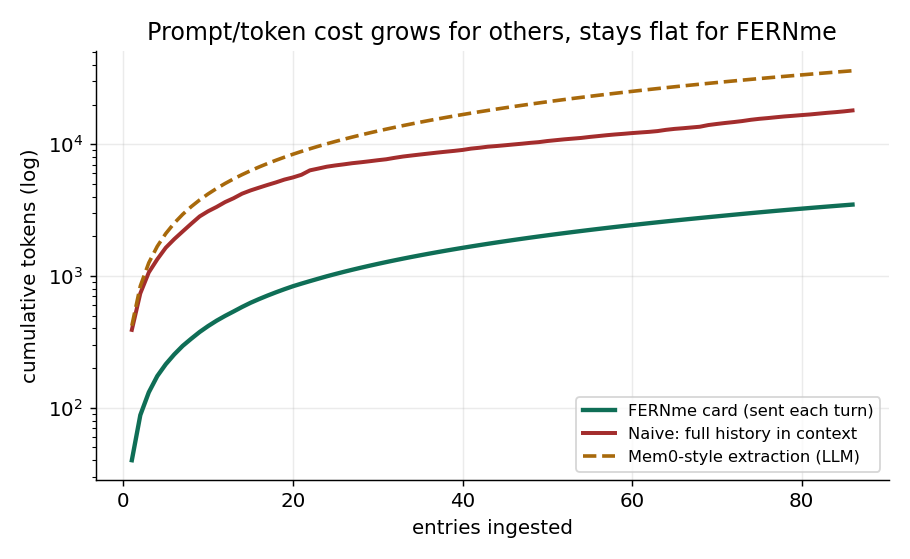
\includegraphics[width=0.82\linewidth]{01_cost_growth.png}
\caption{Cumulative tokens (log): FERNme stays low and flat while naive history and
extraction grow.}\label{fig:cost}
\end{figure}

\begin{figure}[t]\centering
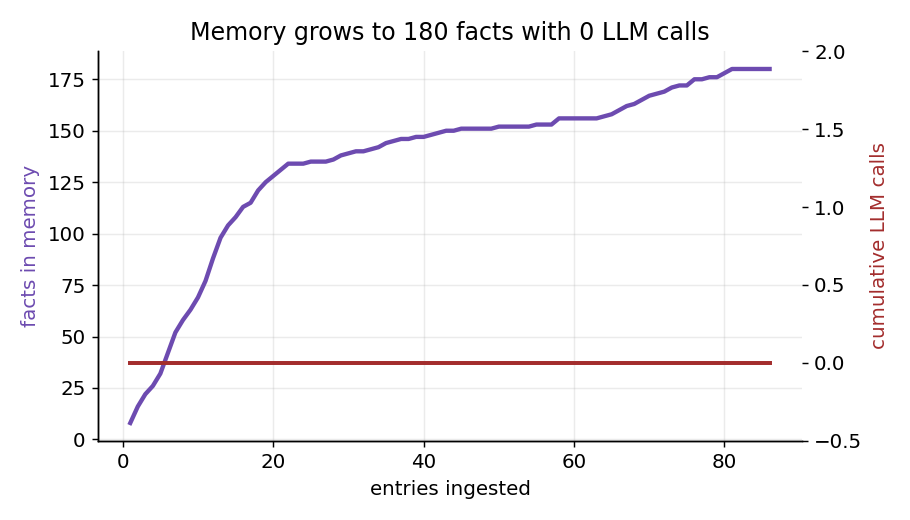
\includegraphics[width=0.82\linewidth]{03_growth_zero_llm.png}
\caption{Memory climbs to 180 facts while the write-path LLM-call count stays pinned at
$0$.}\label{fig:growth}
\end{figure}

\begin{figure}[t]\centering
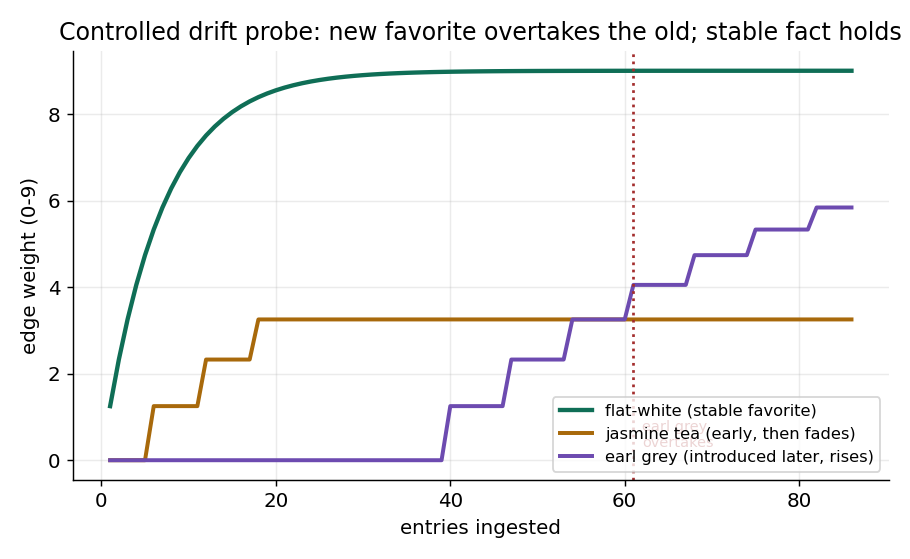
\includegraphics[width=0.82\linewidth]{04_drift.png}
\caption{Controlled drift probe following the diary narrative: a newly introduced favorite
(earl grey) overtakes the old one (jasmine) under decay, while a stable favorite holds.}
\label{fig:drift}
\end{figure}

\begin{figure}[t]\centering
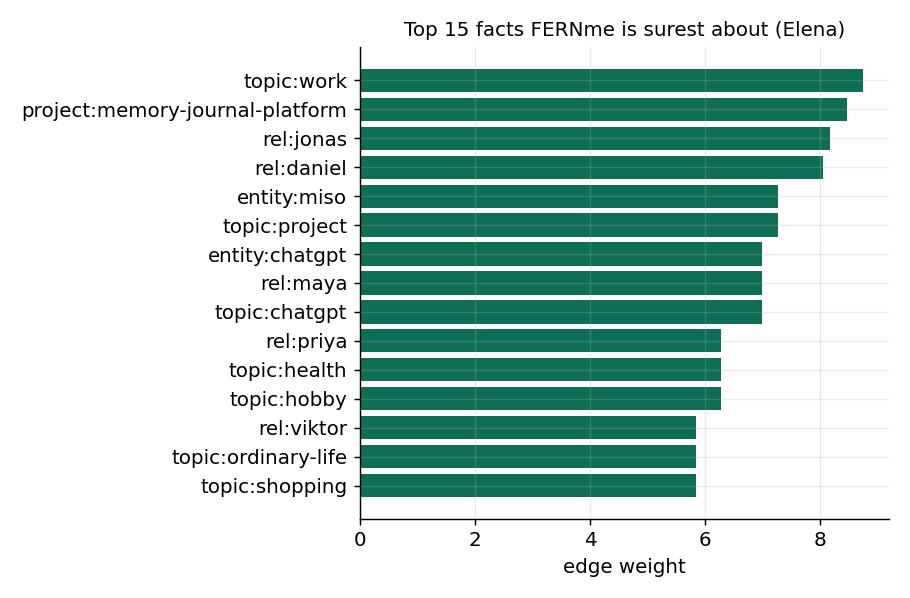
\includegraphics[width=0.82\linewidth]{07_top_hubs.png}
\caption{The 15 facts FERNme is surest about --- the person's real anchors.}\label{fig:hubs}
\end{figure}

\paragraph{What this proves, precisely.} This validates FERNme's \emph{memory mechanics}
--- storage, reinforcement, decay, confidence calibration, drift, associations, and flat
cost --- on realistic long-form single-user data. It does \emph{not} prove answer-quality
parity with an LLM memory: the tag extraction was done by the agent/parser, so fact
coverage is high by construction, and Figure~\ref{fig:drift} is a controlled probe.

\subsection{Head-to-head QA (LoCoMo-style)}\label{sec:qa}
We turn the Elena memory into a question-answering benchmark: 33 fact questions spanning
identity, preferences, relationships, goals/projects, negation, health, and a
\textbf{drift} case (``which tea does she reach for in the afternoon \emph{now}?'').
Following the retrieval-proxy convention (with the right fact retrieved, an LLM answers
correctly), a question is \textbf{answered} if the gold attribute is in the system's
top-$k$ retrieved facts. All compared systems are \textbf{LLM-free and runnable}: FERNme
(context-seeded spreading activation), FERNme without context (weight-only ablation), an
all-time \textbf{frequency} counter, and a \textbf{recency} ranker. A real Mem0 (LLM)
run needs API keys and is \textbf{not run here}; its published LoCoMo scores (single-hop
F1 $\approx 39$, multi-hop $\approx 29$, different dataset, LLM-answered) are noted as
external context, not as a row.

\begin{table}[t]\centering
\caption{LoCoMo-style QA at a matched top-10 budget (${\sim}40$ tokens). FERNme answers
${\sim}4\times$ as many questions as the cheap counters and is the only method to resolve
the drift question.}\label{tab:qa}
\begin{tabular}{lrrrr}
\toprule
system & accuracy & drift & projects & relationships\\
\midrule
\textbf{FERNme (context)} & \textbf{36.4\%} & \textbf{100\%} & \textbf{100\%} & \textbf{67\%}\\
FERNme (no context) & 9.1\% & 0\% & 50\% & 33\%\\
Frequency & 9.1\% & 0\% & 50\% & 33\%\\
Recency & 3.0\% & 0\% & 0\% & 17\%\\
\bottomrule
\end{tabular}
\end{table}

The absolute number is held down by the harsh budget (top-10 of ${\sim}170$ facts) and the
coarse, agent-side tag extraction --- not the retrieval: a budget sweep
(Figure~\ref{fig:sweep}) shows FERNme climbing to $76\%$ at top-20 and ${\sim}91\%$ at
top-30, while frequency/recency plateau near $42\%$ / $27\%$.

\begin{figure}[t]\centering
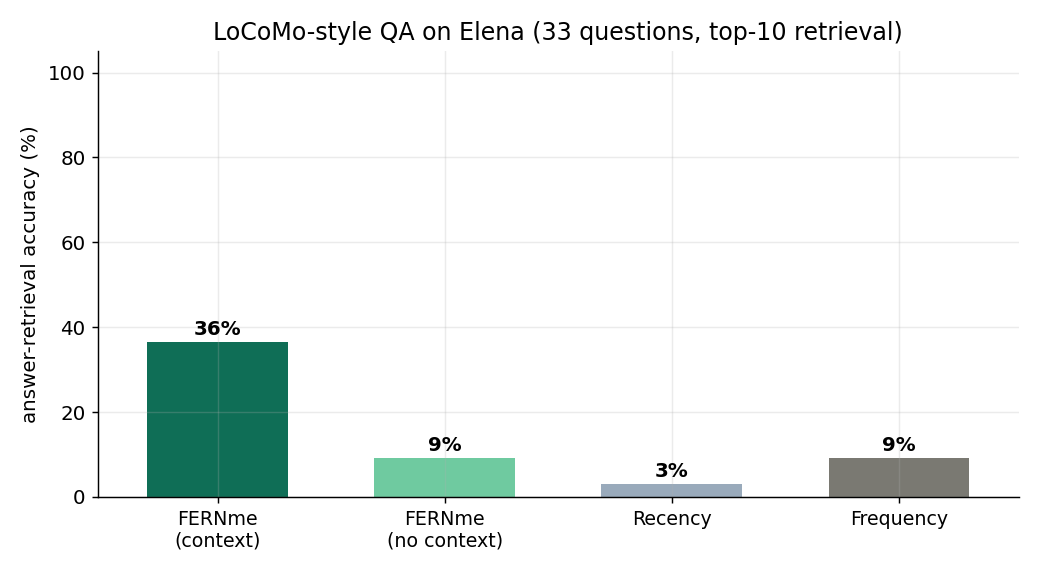
\includegraphics[width=0.82\linewidth]{09_qa_accuracy.png}
\caption{Answer-retrieval accuracy at top-10: context-seeded FERNme vs.\ LLM-free
baselines.}\label{fig:qaacc}
\end{figure}

\begin{figure}[t]\centering
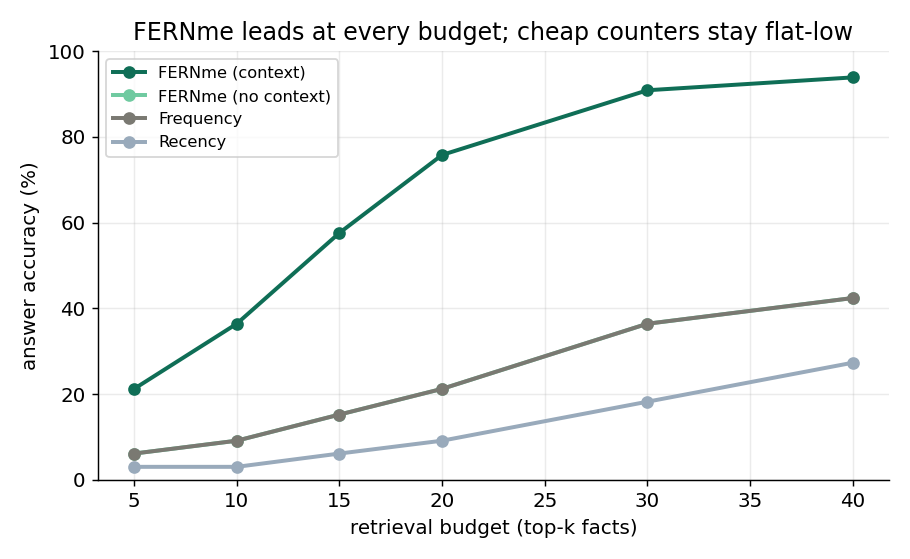
\includegraphics[width=0.82\linewidth]{11_qa_budget_sweep.png}
\caption{Accuracy vs.\ retrieval budget: FERNme leads at every $k$ and converges toward
near-perfect recall; cheap counters stay flat-low.}\label{fig:sweep}
\end{figure}

This is a head-to-head among \emph{LLM-free} memories on real free-form text, at equal
token budget --- exactly the regime FERNme targets. It does not yet establish parity with
an LLM memory (Mem0) on free-text answer quality; that billed comparison remains the
single open experiment.

\subsection{Salience-modulated forgetting}\label{sec:salience}
FERNme's weight is frequency/recency-driven, so a rare-but-intense signal would normally
fade. An optional per-edge \textbf{salience} slows decay,
$\lambda_\mathrm{eff}=\lambda(1-\beta s)$, fed by behavioral significance rather than an
LLM. Figure~\ref{fig:salience} shows two signals seen once at equal strength: the
significant one (intensity $1.0$) stays above the forget threshold for months while the
neutral one is dropped. Salience controls \emph{retention}, not \emph{action} (confidence
still gates acting), so a single strong complaint is remembered but verified before use.
It is off by default ($\beta=0$), so it changes none of the results above unless enabled.

\begin{figure}[t]\centering
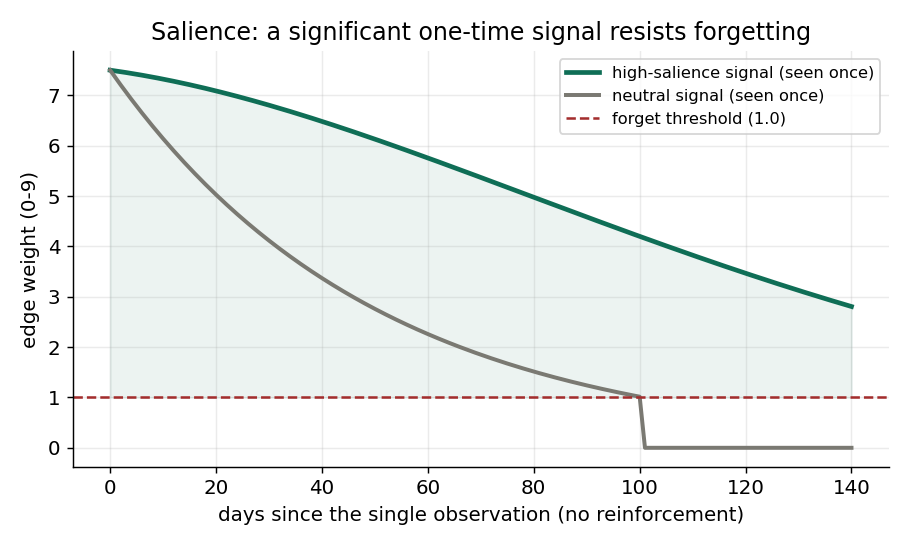
\includegraphics[width=0.82\linewidth]{12_salience.png}
\caption{A significant one-time signal resists forgetting; a neutral one fades below the
forget threshold.}\label{fig:salience}
\end{figure}

\section{Discussion}
On static recall a cheap counter is hard to beat --- so the case for FERNme is not
superior stationary accuracy; it is cost plus robustness. FERNme's advantage appears
exactly where a counter is weak: non-stationarity and context. Decay supplies adaptivity
that frequency lacks, and spreading activation supplies context-sensitivity that neither
frequency nor recency has, while retaining frequency's stability on static data. The Elena
evaluation shows these mechanics also hold on free-form text.

\section{Limitations}
\begin{itemize}[leftmargin=1.4em,itemsep=2pt]
\item \textbf{Simulation + one synthetic person, not a human study.} Synthetic results
define their own ground truth; the Elena dataset is realistic but fictional and its
extraction is agent/parser-driven.
\item \textbf{Nuance gap.} A co-occurrence counter misses causal/contextual preferences an
LLM extractor catches; the Mem0 head-to-head that would quantify this is not yet run.
\item \textbf{Mapping dependency.} The no-LLM write depends on catalog/vocabulary quality;
thin-metadata surfaces degrade to coarse attributes.
\item \textbf{Token figures are estimates} (chars/4; tiktoken's vocabulary was unavailable
offline), cross-checked by word count.
\item \textbf{Tuning and granularity.} Spreading-activation parameters are hand-set;
single-digit fuzzy weights lose fine degree.
\end{itemize}

\section{Ethics and broader impact}
FERNme stores personal data, including potentially sensitive signals. Its design choices
are protective: per-tenant isolation, consent gating, glass-box edit/export/delete, a
tamper-evident audit chain, $k$-anonymity and differential privacy on the shared prior, and
a cross-surface supernode that is user-owned and default-deny --- aggregation by and for the
user, never covert cross-site tracking. We explicitly exclude inferring or acting on user
vulnerability. These are mitigations, not guarantees; deployments handling regulated data
require legal review.

\section{Conclusion}
For agents that act on people's behalf, memory should be cheap to write, bounded in cost,
evaluated by outcomes, and owned by the user. FERNme demonstrates that a no-LLM Hebbian
write over a fuzzy preference graph, with differential encoding and spreading-activation
retrieval, delivers flat-cost, interpretable, per-surface memory that is robust where cheap
baselines fail, that lifts a simulated outcome metric, and that builds a coherent profile
from 86 entries of free-form text at near-zero write cost.

\paragraph{Reproducibility.} Code, tests (88 passing, including a real-Postgres backend),
and every experiment are in the repository (\url{https://github.com/mirkofr/FERNme}). Run
\texttt{python -m fernme.eval.<name>} for each simulation result, \texttt{python demo/elena/eval\_elena.py}
for Section~\ref{sec:elena} and \texttt{python demo/elena/eval\_elena\_qa.py} for Section~\ref{sec:qa}.

\begin{thebibliography}{9}
\bibitem{hipporag} B.~J. Guti\'errez, Y.~Shu, Y.~Gu, M.~Yasunaga, Y.~Su.
\emph{HippoRAG: Neurobiologically Inspired Long-Term Memory for Large Language Models.}
NeurIPS, 2024. arXiv:2405.14831.
\bibitem{hipporag2} B.~J. Guti\'errez, Y.~Shu, W.~Qi, S.~Zhou, Y.~Su.
\emph{From RAG to Memory: Non-Parametric Continual Learning for LLMs.} ICML, 2025.
arXiv:2502.14802.
\bibitem{mem0} Mem0: Building Production-Ready AI Agents with Scalable Long-Term Memory.
2025. arXiv:2504.19413.
\bibitem{helamem} J.~Zhu, J.~Li, C.~Zhang, J.~Liu, M.~Yang.
\emph{HeLa-Mem: Hebbian Learning and Associative Memory for LLM Agents.} 2026.
arXiv:2604.16839.
\bibitem{ori} Ori-Mnemos: Local-first persistent agentic memory.
\url{https://github.com/aayoawoyemi/Ori-Mnemos}.
\bibitem{collins1975spreading} A.~M. Collins, E.~F. Loftus.
\emph{A spreading-activation theory of semantic processing.} Psychological Review, 1975.
\bibitem{anderson2004actr} J.~R. Anderson et al.
\emph{An integrated theory of the mind (ACT-R).} Psychological Review, 2004.
\bibitem{hebb1949} D.~O. Hebb. \emph{The Organization of Behavior.} Wiley, 1949.
\bibitem{zadeh1965} L.~A. Zadeh. \emph{Fuzzy sets.} Information and Control, 1965.
\end{thebibliography}

\end{document}
